\subsubsection{Mynstur unnin til að senda á vél}
Byrjað var á því að skrifa kóða sem tekur fylki af tölum sem táknar mynd sem á að prjóna og kemur því yfir á rétt form til að senda á prjónavélina. Litirnir geta verið í mesta lagi fjórir og inniheldur hvert munstur sem sent er á vélina þar með heiltölurnar $1$, $2$, $3$ og $4$ eftir því með hve mörgum litum á að prjóna. Sérhver $1$ í munstrinu táknar eina lykkju sem á að prjóna með lit eitt, $2$ táknar lykkjur sem prjóna á með lit t o.s.frv. Talan $0$ táknar óprjónaðar lykkjur. 

Vélin prjónar með aðeins einum lit í einu og prjónar tvær umferðir áður en skipt er um lit. Ef prjónað er með fjórum litum tekur því hver lína í munstur fylkinu átta umferðir í vélinni. Skrifað var fall sem tekur inn fylki af tölum og aðskilur tölurnar í mismunandi lista þar sem fyllt er upp í með núllum og þ.a. hver listi kemur tvisvar sinnum fyrir (þar sem í fyrst fer sleðinn frá hægri til vinstri og svo fer sleðinn vinstri til hægri). 

\textbf{Dæmi}: Ef gefið er eins línu munstrið $$[1,2,2,3,4]$$ skilar fallið lista af listum: 
\[
\left[
\begin{array}{c}
\left[1, 0, 0, 0, 0\right], \left[1, 0, 0, 0, 0\right], \\
\left[0, 2, 2, 0, 0\right], \left[0, 2, 2, 0, 0\right], \\
\left[0, 0, 0, 3, 0\right], \left[0, 0, 0, 3, 0\right], \\
\left[0, 0, 0, 0, 4\right], \left[0, 0, 0, 0, 4\right]
\end{array}
\right]
\]
Á mynd \ref{fig:litid_prjon} má sjá hvernig einfaldri mynd er lýst með fylki af tölum og svo hvernig prjónamunstrið sem sent er á vélina lítur út ef prjóna á myndina.

\begin{figure}
    \centering
    
\includegraphics[height=.3\textheight]{myndir/snaeja/litid_prjon_fyrir.png}
    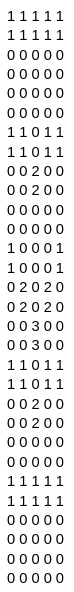
\includegraphics[height=.3\textheight]{myndir/snaeja/litid_prjon_separated.png}
    \caption{Til hægri má sjá einfalt prjónamunstur í þremur litum þar sem hver heiltala táknar eina lykkju í ákveðnum lit. Til vinstri hvernig sama munstur lítur út áður en það er sent á vélina.}
    \label{fig:litid_prjon}
\end{figure}

\subsubsection{Íslenska Sjónabókin nýtt í mynsturgerð}
Íslenska Sjónabókin inniheldur útsaums munstur úr þeim sjónabókum sem varðveist hafa á Íslandi. Með \textit{Íslensku Sjónabókinni} fylgir geisladiskur með öllum þeim síðum af munstrum sem í henni eru. Skrárnar eru ýmist á \texttt{.pdf} eða \texttt{.eps} formi og henta illa til að vinna með í tölvu. Til að nýta munstrin og senda þau á prjónavélina þurfti að koma þeim á annað og betra stafrænt form. Langflest munstrin í bókinni eru í tveimur litum þ.e. kross og ekki kross og því var einskorðað á þau í þessum hluta verkefnisins.

Skrifaður var kóði sem settur var á GitHub\footnote{Kóðinn og mynstrin má finna á \url{https://github.com/HiDefTextiles/Sjonabok}.} þ.a. hver sem getur sótt kóðann og notað mynstrin á handhægara formi. Kóðinn virkar þannig að hver \texttt{.eps} skrá er sótt og sett í grátóna fylki í Python. Fylkinu er svo skipt í núll og einn þannig að hver pixill sem er yfir ákveðinn þröskuld af dökkum gráum er látinn vera svartur ($1$) og restin er sett sem hvítur($0$). Síðan eru rúðustrikuðu línurnar fundnar og innan hvers reits ef hlutfall svartra pixla er yfir $0.5$ er litið á sem svo að kross sé inni í reitinum. Þessum upplýsingum er svo safnað saman í nýtt fylki þar sem $1$ stendur fyrir kross og $0$ engan kross. Öllu auka plássi fyrir utan munstrið er síðan hent og fylkið vistað á tveimur skráarsniðum, texta sniði og \texttt{.png} sniði. Texta skránum er einfalt að hlaða inn í fylki til að nota síðar og þægilegra er að skoða munstrin á \texttt{.png} sniði. Á mynd \ref{fig: sjonabok_munstur} má sjá hvernig munstur lítur út eftir vinnslu. 


\begin{figure}
    \centering
    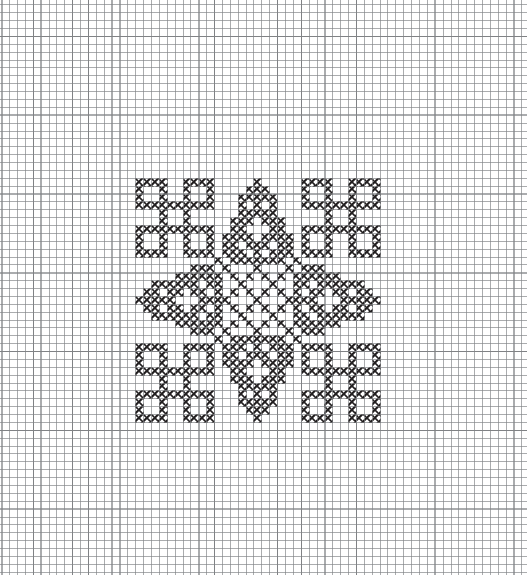
\includegraphics[height=.3\textheight]{myndir/snaeja/sjonabok_before.png}
    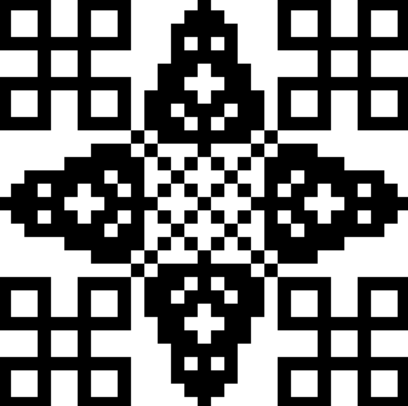
\includegraphics[height=.3\textheight]{myndir/snaeja/sjonabok_after.png}
    \caption{Til hægri má sjá munstur úr \textit{Íslensku Sjónabókinni} í \texttt{.eps} skrá. Til vinstri hvernig sama munstur lítur út eftir vinnslu á \texttt{.png} formi.}
    \label{fig: sjonabok_munstur}
\end{figure}

Í sumum skrám er fleira ein eitt munstur að finna. Til að geta nýtt þau þarf að aðskilja þau. Borða er einfalt að aðskilja þar sem þeir aðskiljast alveg einungis lárétt eða lóðrétt. Önnur munstur og stafróf aðskiljast á flóknari máta og var útfærlsa af DFS nýtt til að aðskilja þau. Aðskilin munstur eru svo vistuð sér þ.a. ein síða af munstrum fara í sömu möppu. Einnig var skrifaður kóði sem finnur endurtekningar í munstri og geymir þá minnstu endurtekninguna.

Skrifuð voru nokkur föll fyrir munsturgerð í Python. Eitt af þeim var fall sem breytir myndum (\texttt{.jpg} eða \texttt{.png}) í prjónamynstur. Fallið tekur inn vísun á myndaskrá, hversu margar lykkjur munstrið á að vera og fjölda lita. Fallið gráskalar myndina, fækkar pixlum í samræmi við fjölda lykkja og notar síðan Floyd-Steinberg reikniritið til að fækka litum \cite{FloydSteinberg}. Fallið skilar svo fylki af heiltölum á bilinu $1$ til $4$ þar sem $1$ táknar ljósustu pixlana á grátóna bilinu og hæsta talan þá dekkstu. Sökum þess hvernig Floyd-Steinberg reikniritið virkar að ef bakgrunnur einhverrar myndar er aðeins í einum lit endar hann oft á að innihalda staka pixla í dekkri lit eftir að því er beitt á myndina. Því var skrifað reiknirit sem tekur svoleiðis staka pixla og breytir þeim í sama lit og aðalbakgrunnslitinn. Við gerð þessa reiknirits var \textit{flood fill} reikniritið nýtt.

Önnur föll sem nýta sjónabókamunstrin voru einnig skrifuð. Eitt þeirra bætir við borða umhverfis prjónamunstur eftir óskum notendans (mynd \ref{fig: sjonabok_bordi}). Annað gerir kleift að skrifa texta með sjónabókar leturgerðum eins og sjá má á mynd \ref{fig:hallo_heimur}. Textinn getur ýmist verið  miðjaður eða vinstri jafnaður. Skrifað var fall sem bætir við sjónabókarmunstri sem bakgrunni við munsturfylki (mynd \ref{fig:raggajóns}). Það fall nýtir \textit{flood fill} reikniritið. Fallið var útfært þannig að ef mynd er prjónuð og bakgrunnur bættur við hana getur næsta mynd sem er prjónuð einnig haft sama bakgrunn og þannig að bakgrunnarnir renna saman í einn heildstæðan bakgrunn þ.e. ekki sjást skil í bakgrunninum á milli myndanna tveggja.

\begin{figure}[p]
    \centering
    \begin{minipage}[b]{0.45\linewidth}
        \centering
        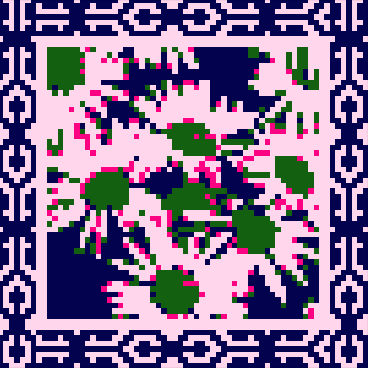
\includegraphics[width=.8\linewidth]{myndir/snaeja/bordi.png}
        \caption{Borða úr \textit{Íslensku Sjónabókinni} bætt við í kringum prjónamynstur. Prjónamynstrið er í 4 litum og kemur frá ljósmynd af baldursbrám.}
        \label{fig: sjonabok_bordi}
    \end{minipage}
    \hspace{0.05\linewidth} % Add space between the figures
    \begin{minipage}[b]{0.45\linewidth}
        \centering
        \includegraphics[width=\linewidth]{myndir/snaeja/raggajóns.png}
        \caption{Prjónamynstur af Ragnheiði Jónsdóttur með mynstur úr \textit{Sjónabók} sem bakgrunn.}
        \label{fig:raggajóns}
    \end{minipage}
\end{figure}

\begin{figure}[p]
    \centering
    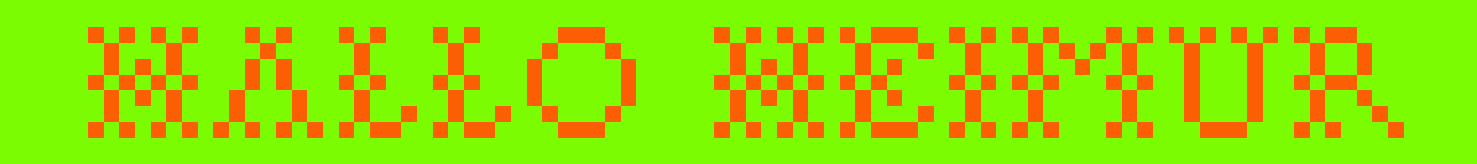
\includegraphics[width=0.5\linewidth]{myndir/snaeja/hallo_heimur.png}
    \caption{\textit{Halló heimur} prjónamynstur skrifað með letri úr \textit{Sjónabók}.}
    \label{fig:hallo_heimur}
\end{figure}

\subsubsection{Ókláruð verkefni}
Aðrar aðferðir voru prófaðar fyrir mynstur gerð. \textit{Wave Function Collapse} (WFC) reikniritið var sett upp með hnútum sem finna má á mörgum stöðum í \textit{Íslensku Sjónabókinni}. Ákveðið var þessi munsturgerð myndi ekki henta í hönnunarvinnuna að svo stöddu og því var ekki kafað dýpra ofan í WFC en á mynd \ref{fig:wfc} má sjá útkomu úr reikniritinu. Einnig var byrjað á að þróa aðferð sem litar munstur úr sjónabókinni sjálfvirkt í 3 til 4 litum. Sökum tímahraks tókst ekki að klára þá vinnu en var hún komin nokkuð áleiðis og mætti halda áfram með hana síðar.

\begin{figure}[p]
    \centering
    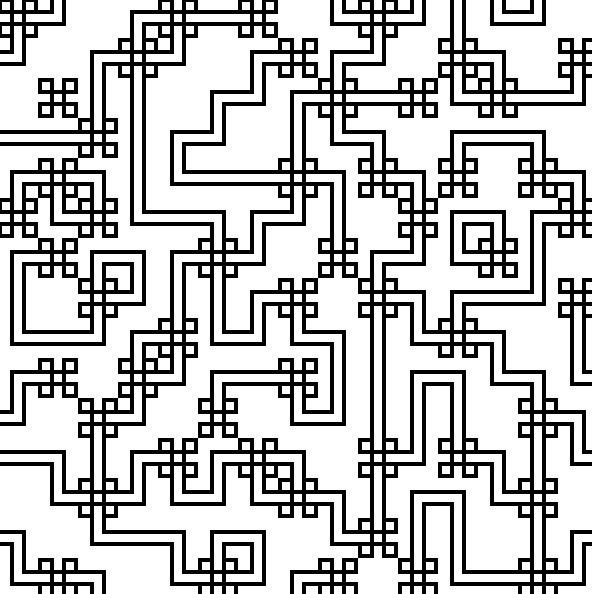
\includegraphics[width=0.5\linewidth]{myndir/snaeja/wfc.png}
    \caption{\textit{Wave Function Collapse} reikniritið notað til að búa til prjónamunstur. Hnúturinn í munstrinu finnst á mörgum stöðum í \textit{Íslensku Sjónabókinni} en dæmi um hann er á mynd \ref{fig: sjonabok_munstur}.}
    \label{fig:wfc}
\end{figure}
